\section{Electron and Photons}
\label{sec:reco:EM}

\subsection{Electron and Photon Reconstruction}
\label{sec:EM:reco}

\indent Both electron and photon reconstruct start from clusters of energy deposits in the electromagnetic calorimeter.  The EM calorimeter is first divided into a grid of towers each with the size of $\Delta \eta \times \Delta \phi = 0.025 \times 0.025$.  The energy from all longitudinal layers inside each tower is summed into the total tower energy.  \\

\indent The EM clusters are seeded by towers with energy above a certain threshold.  A sliding-window algorithm groups energy towers near the seed into EM clusters.\cite{EMReco13TeV,EMReco8TeV}  The window width is $3 \times 7$ towers in the barrel and $5 \times 5$ towers in the endcap.  The reconstructed cluster therefore has a size of $\Delta \eta \times \Delta \phi = 0.075 \times 0.175$ in the barrel and $ 0.125 \times 0.125$ in the endcap.  The same window size is used for electrons and photons to ensure better cancelation of systematics when using electrons to the measure photon response.\cite{EMReco13TeV}  The window position is adjusted so that the reconstructed cluster energy is the local maximum.  The different cluster sizes were optimized for the different energy distribution in the barrel and endcap calorimeters while minimizing pileup and noise contributions.\cite{EMReco13TeV}  \\

\indent Identified clusters are then matched to reconstructed ID tracks using the track and cluster position.  ID tracks are required to have a minimum number of pixel and total silicon hits.  Clusters are considered an electron candidate if a single well-reconstructed ID track with an associated vertex is found.  The cluster is considered an unconverted photon candidate if no tracks are found.  The cluster is considered a converted photon candidates if two opposite signed collinear tracks which are consistent with electrons are present.  The cluster if also considered a converted photon if a single track is present but the track lacks hits in the IBL of the pixel detector.  \\

\indent Furthermore, electron and photon candidates must satisfy a set of criteria.  These variables include descriptions of the EM shower shapes, amount of hadronic activity behind the EM calorimeter and properties of associated tracks.  More details on electron and photon identification are given in section \ref{sec:reco:eleQuality} and \ref{sec:reco:phoQuality}. \\

\indent A schematic of the electron reconstruction algorithm can be found in figure \ref{fig:elec_reco}. \\

\begin{figure}[!hp] 
\begin{center}
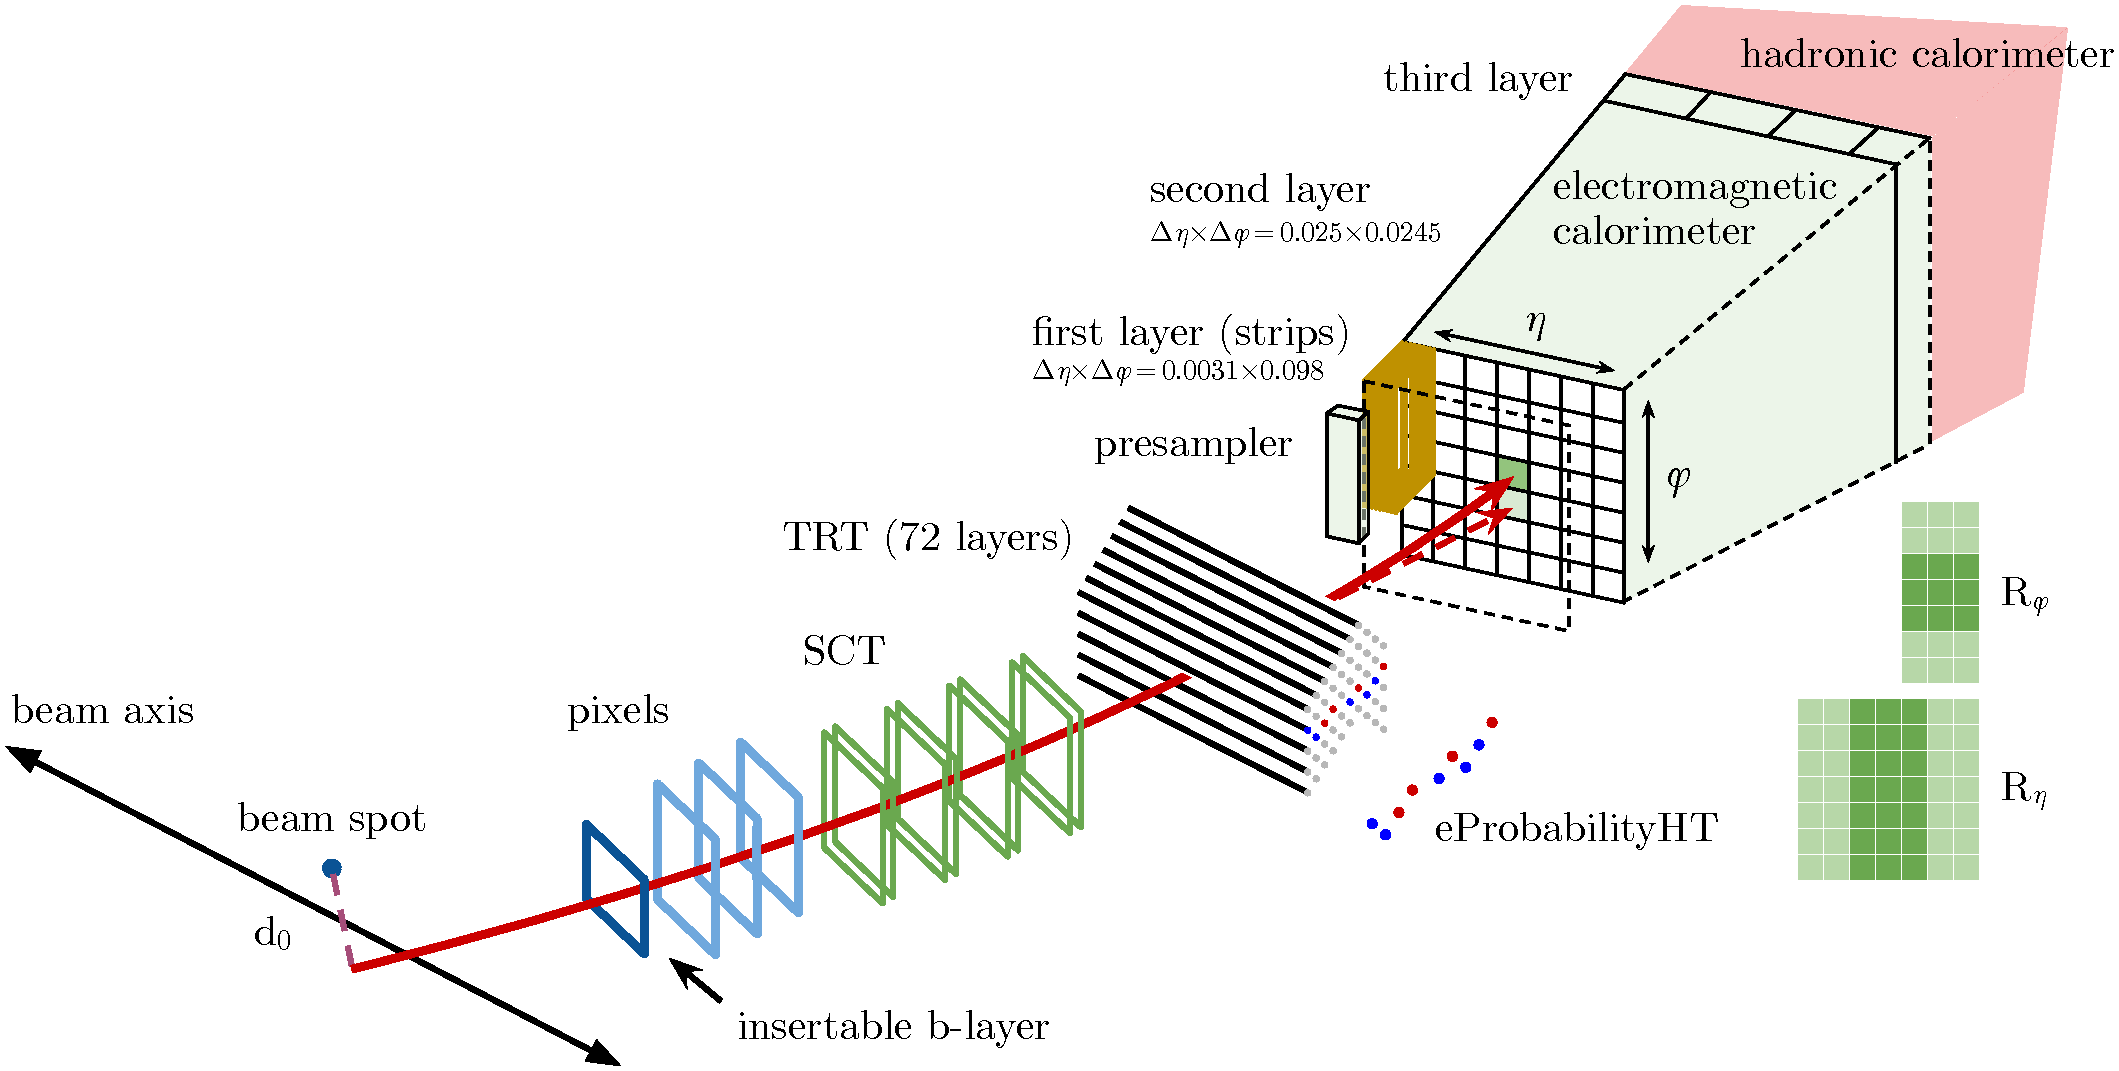
\includegraphics[width=0.65\textwidth]{figures/EMCalib/Reco_Diag.png}
\caption{Schematic representation of the electron reconstruction algorithm. (Figure taken from \cite{EleID}) }
\label{fig:elec_rec}
\end{center}
\end{figure}

\subsection{Electron Identification and Quality}
\label{sec:reco:eleQuality}

\indent Electron identification in Run 2 is based on a likelihood algorithm that depends on a list of kinematics variables including EM shower shape, EM vs hadronic activity ratio, activity in the TRT and properties of the associated track.  The list of variables included in the likelihood can be found in \cite{EleID}.  A multivariate technique is used to ensure the PDF estimation is robust in low statistics regions in the high dimensional space.\cite{TMVA}  Probability density functions (PDF) are formed for electrons and non-electron backgrounds for a set of discriminating variables used on MC.  The probability of the candidate being an electron is calculated using the two PDFs.  \\

\indent Electron identification is split into categories {\it very loose, loose, medium, } and {\it tight}.  Each operating point is a sub-set of another.  For example, all tight electrons are also medium electrons and all medium electrons are also loose electrons.  Because some shower shape distributions tend to broaden with the number of pileup collisions, the cut on the likelihood discriminant is loosened as a function of the number of vertices. This is done to preserve the identification efficient at high pileup and does not drastically increase the amount of background.\cite{EleID}  \\

\indent The electron identification efficiency for the different electron qualities are shown in figure \ref{fig:elec_eff}.  25 GeV tight electrons have an efficiency of 78 percent and fake rate of 0.3 percent.  25 GeV loose electrons have an efficiency of 90 percent and fake rate of 0.8.  The efficiency increases with $E_T$ while the fake rate decreases.\cite{EleID} \\

\begin{figure}[!hp] 
\begin{center}
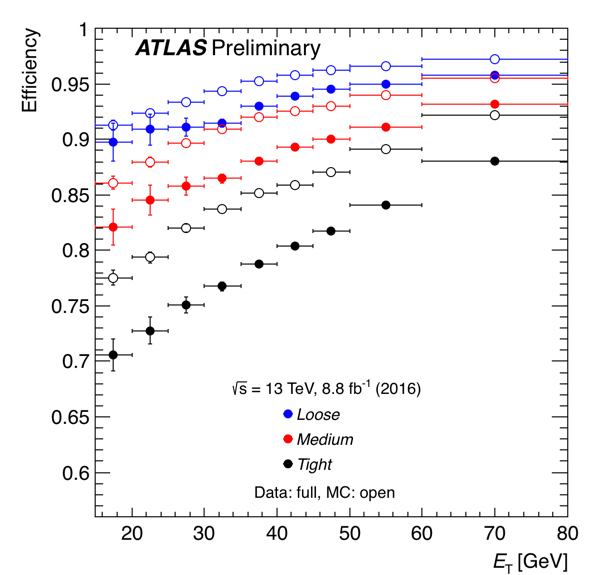
\includegraphics[width=0.45\textwidth]{figures/EMCalib/Elec_Et.png}
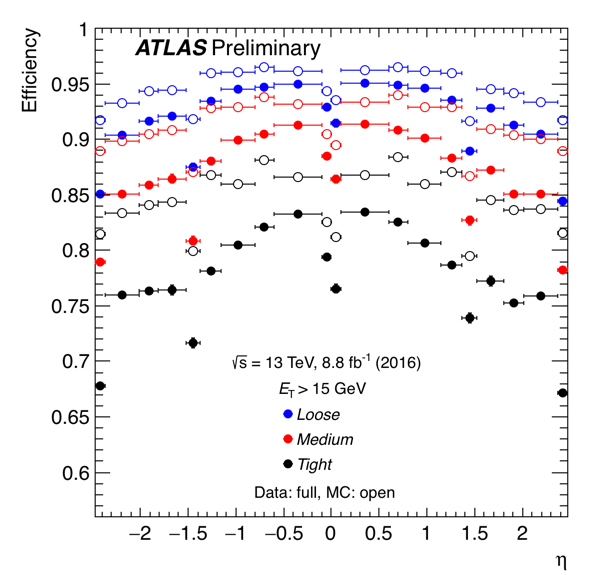
\includegraphics[width=0.45\textwidth]{figures/EMCalib/Elec_eta.png}
\caption{Electron identification efficiency in 2016 data as a function of $E_t$ and $\eta$ for different electron qualities. (Figure taken from \cite{EleID}) }
\label{fig:elec_eff}
\end{center}
\end{figure}

\subsection{Photon Identification and Quality}
\label{sec:reco:photoID}

\indent Photon identification is based on the shower shape and the amount of hadronic activity behind the EM cluster.  The energy deposited in the cells in the first and second layer of the EM calorimeter are important for distinguishing the EM shower originating from photons and those originating the neutral mesons such as $\pi_0$. A detailed list of the discriminating variables used can be found in \cite{photonID}. \\

\indent The requirements differ for converted and unconverted photon candidates to account for differences in expected shower shapes.  The requirements also differ according to pseudorapidity intervals to account for the varying amount of material upstream of the calorimeter. These requirements were optimized using a multivariate technique.\cite{TMVA}\\

\indent Two working points are included a loose and a tight selection.  The loose ID exploits the variables only in the EM calorimeter and in the hadronic calorimeter layer and is typically used for the trigger and for background studies.  The tight ID uses the full granularity of the EM calorimeter, including the fine segmentation of the first sampling layer, and tightens requirements on the variables used in the loose selection.  The tight working point is the one generally recommended for physics analysis and photons used in this analysis are tight photons.  \\

\indent Distribution of photon identification efficiency for tight photons are shown in figure \ref{fig:pho_eff}. \\

\begin{figure}[!hp] 
\begin{center}
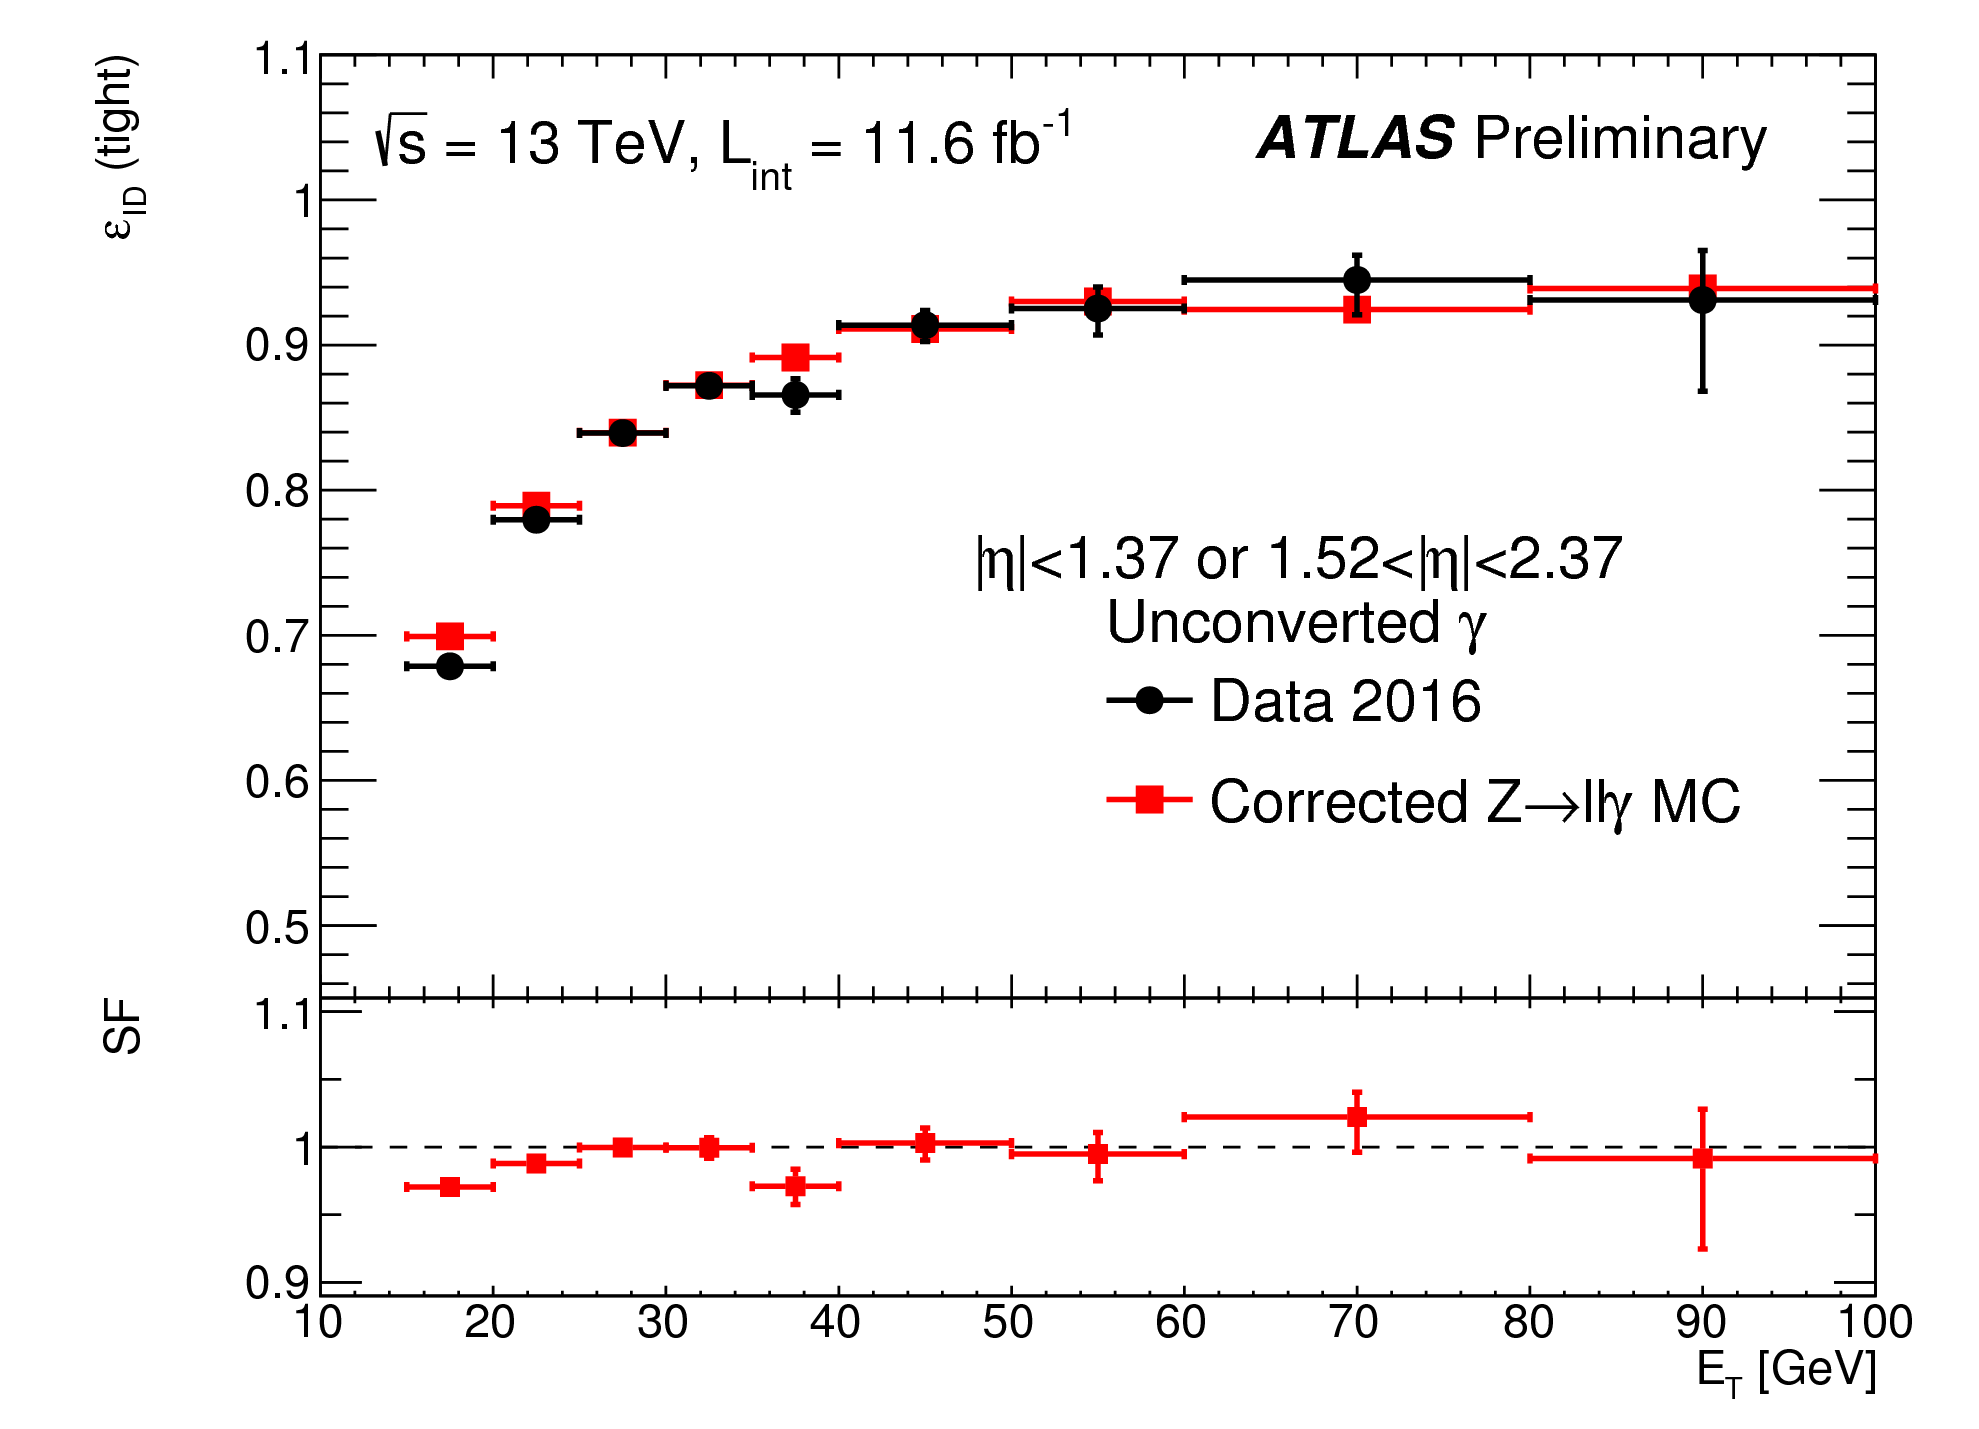
\includegraphics[width=0.45\textwidth]{figures/EMCalib/Unconverted_Et.png}
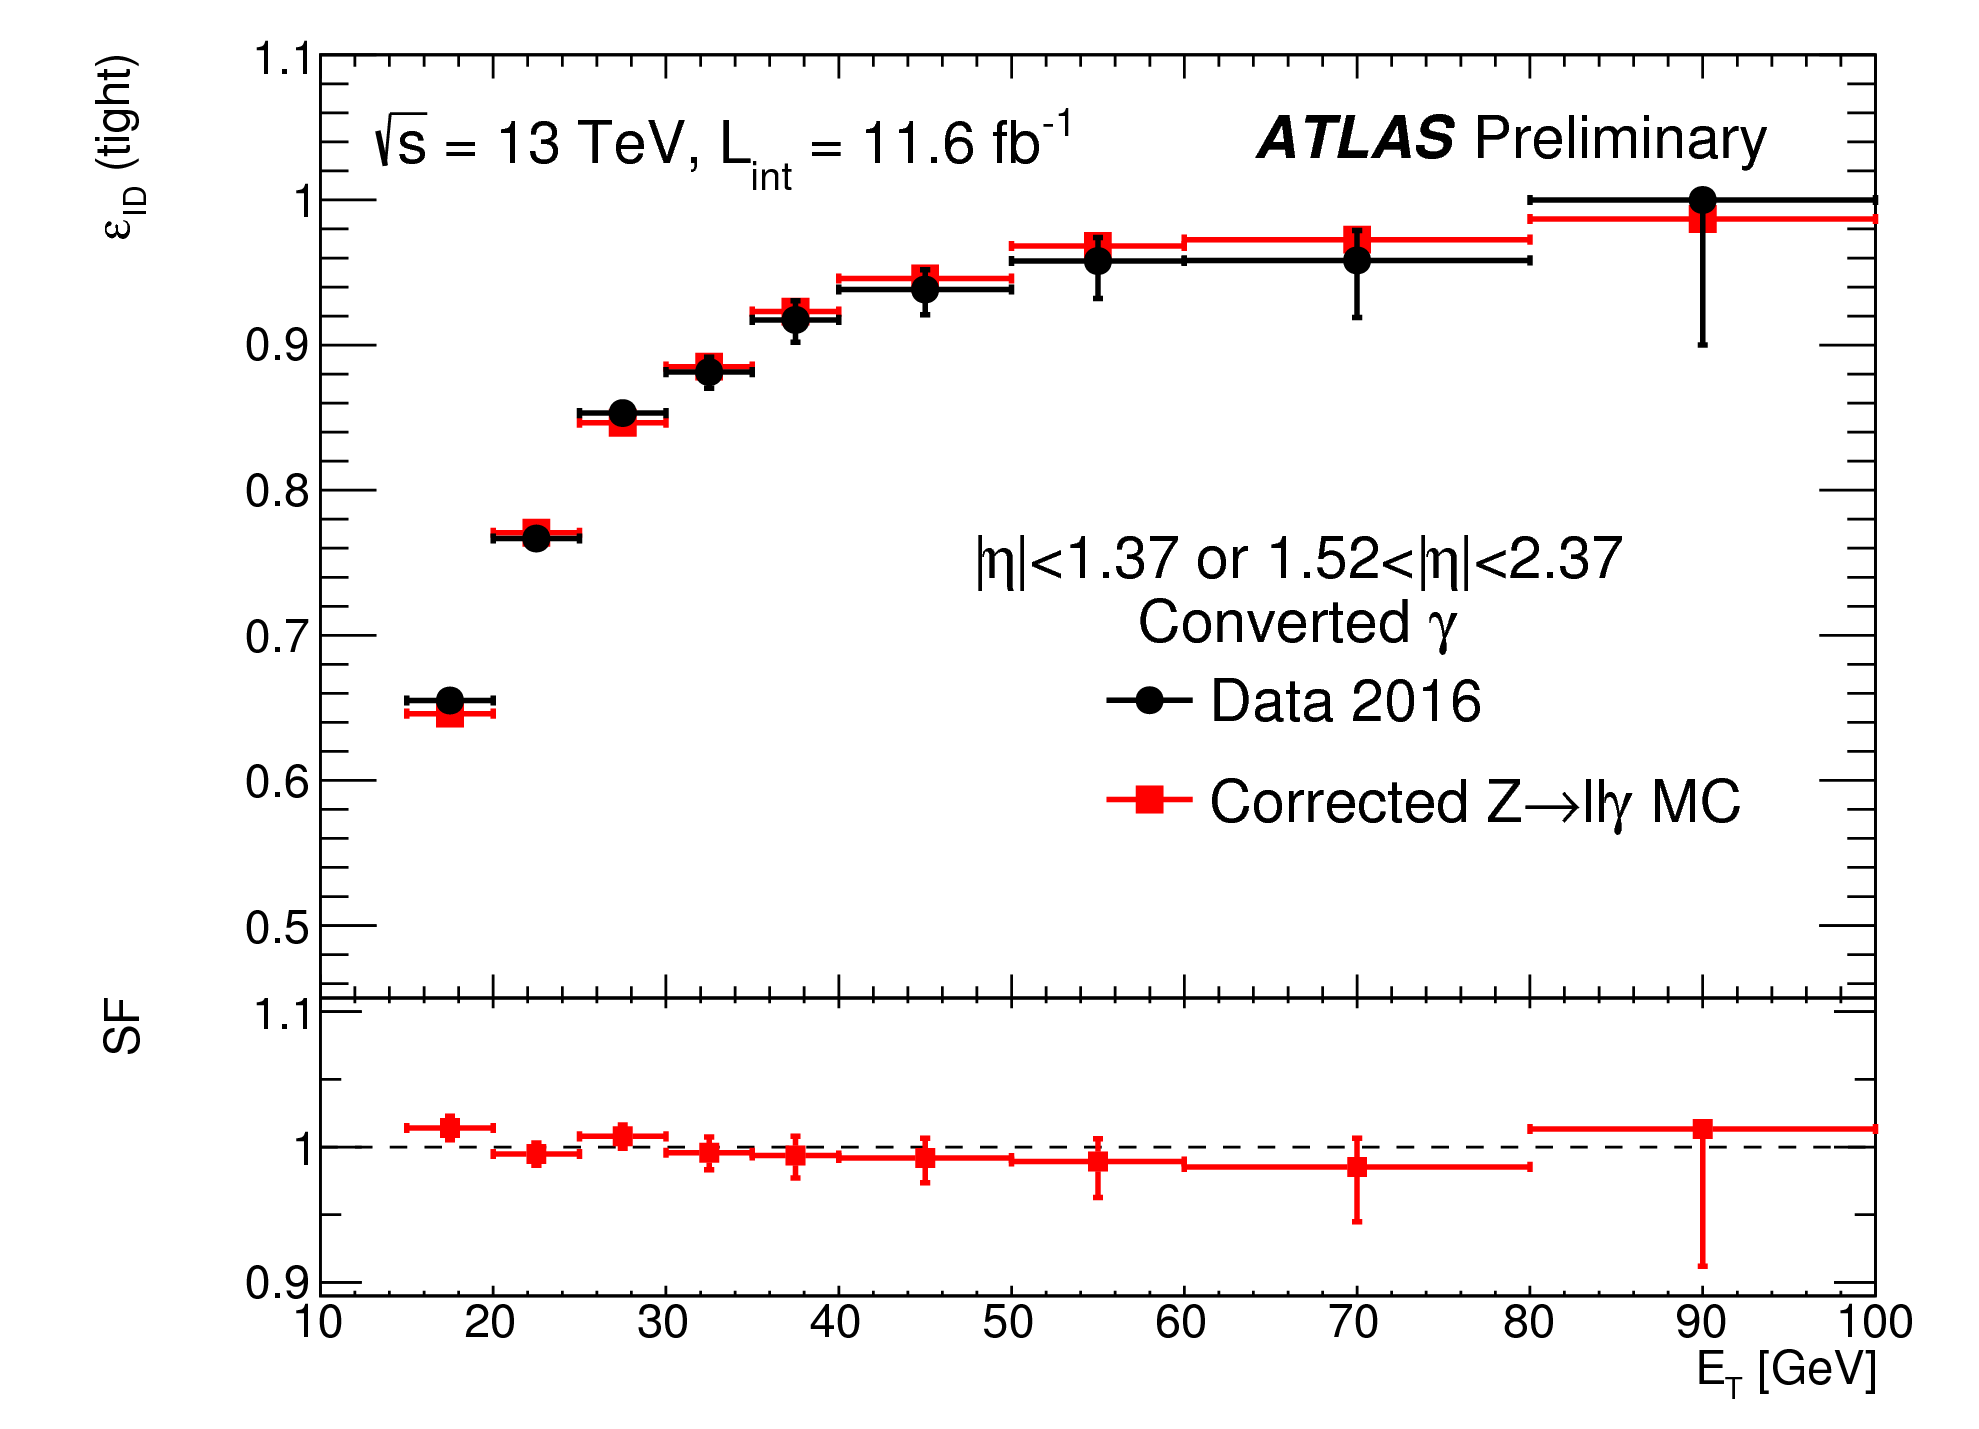
\includegraphics[width=0.45\textwidth]{figures/EMCalib/Converted_Et.png}
\caption{Photon identification efficiency in 2016 data as a function of $E_t$ for converted and unconverted photons. (Figure taken from \cite{EMReco13TeV}) }
\label{fig:elec_eff}
\end{center}
\end{figure}


\subsection{Electron and Photon Energy Calibration}
\label{sec:reco:EMCalibration}

\indent Electron and photon energy must be calibrated because of the sampling nature of the EM calorimeter.  At the same time, correctly estimating the amount of material upstream of the calorimeter is also important.  Typically a $100 \gev$ electron will deposit between a few percent to 20 percent of its energy before it reaches the calorimeter.\cite{EMReco13TeV}  Plus roughly 5 percent of the electron energy may be deposited outside of the cluster.  Electron and photon energy calibration account for all these effects to get an estimate of the true electron and photon energy.  The calibration procedure follow the steps displayed in figure \ref{fig:EMCalibFlow}. \\

\begin{figure}[htb]
  \begin{center}
    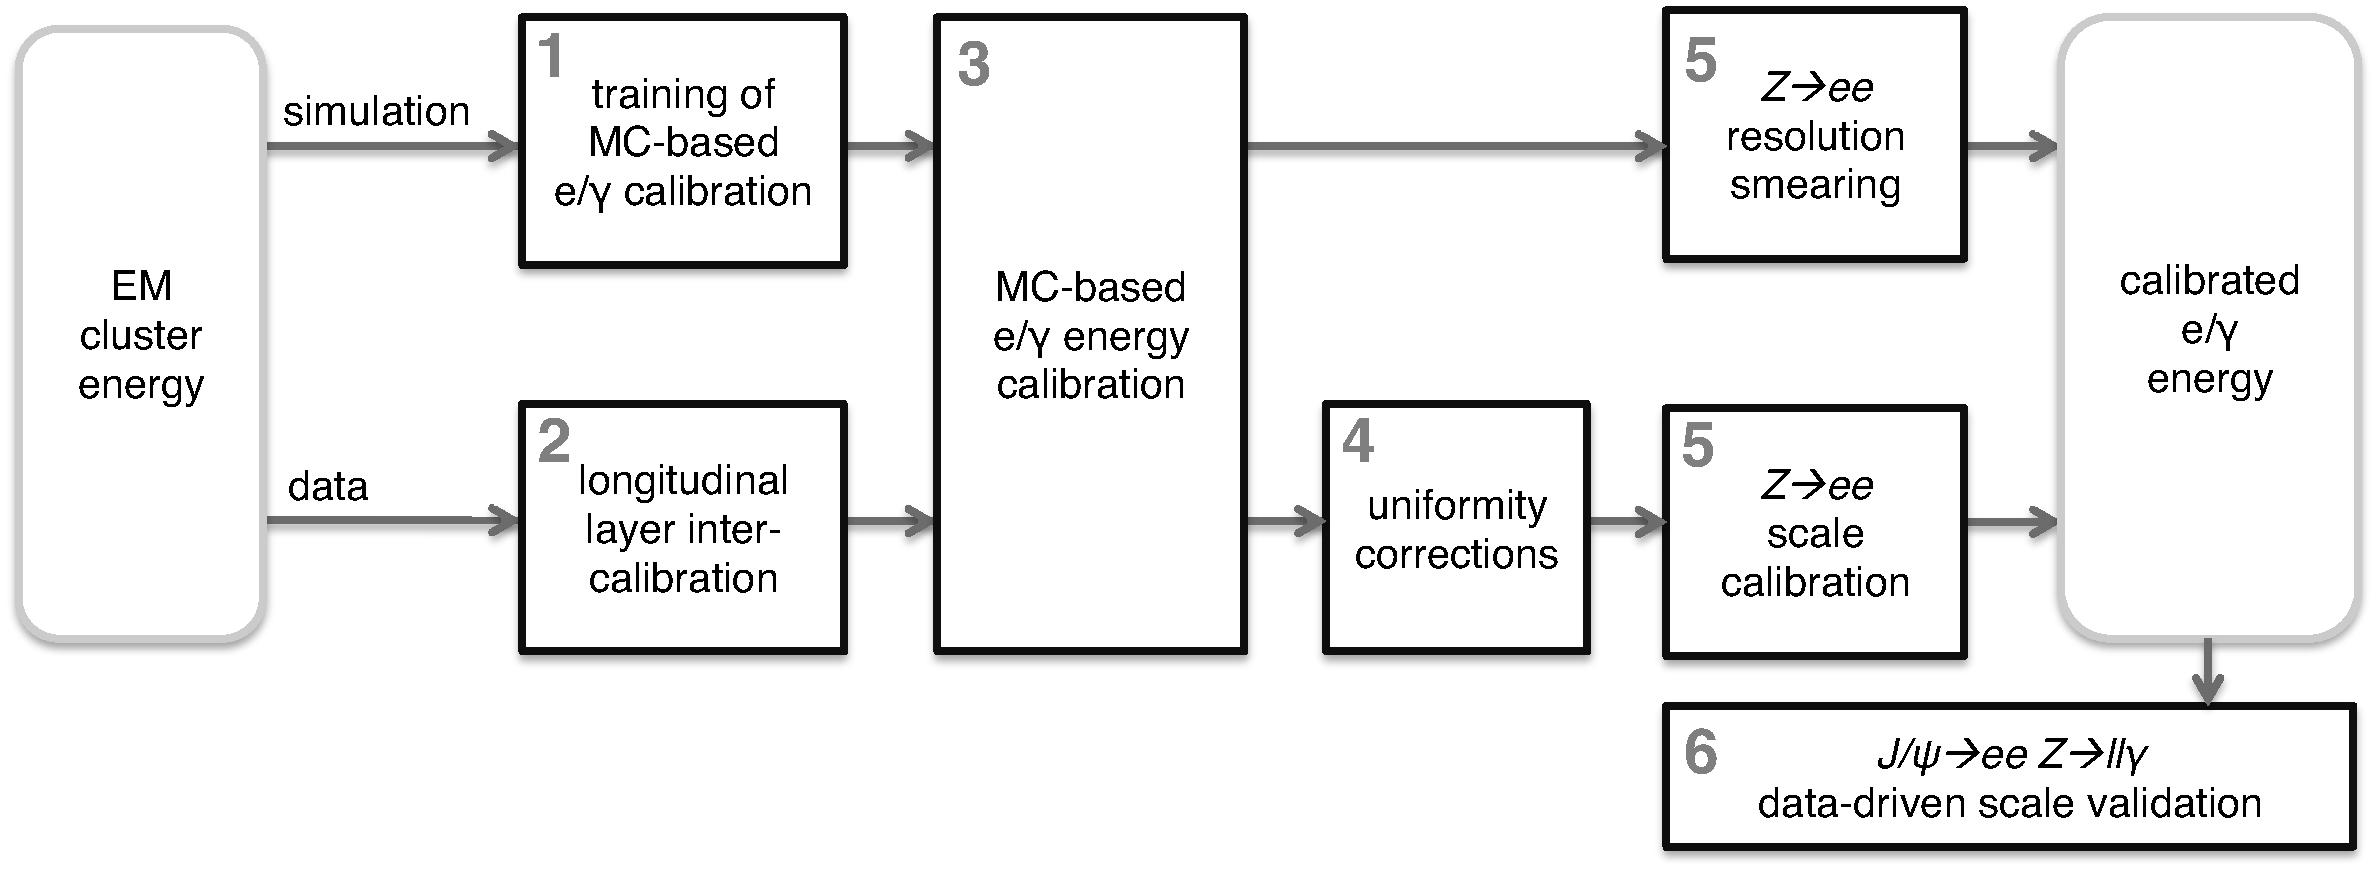
\includegraphics[width=0.85\textwidth]{figures/EMCalib/ElecCalib.png}\hspace{0.05\textwidth}
\end{center}
\caption{Flow chart of the steps involved in the calibration of the energy response of electrons and photons.  (Figure taken from \cite{EMReco8TeV}) }
\label{fig:EMCalibFlow} 
\end{figure}

\indent The EM clusters are first calibrated to the original electron or photon energy using a multivariate technique \cite{TMVA} based on MC simulations.\cite{EMReco13TeV,EMReco8TeV}   The MC based calibration uses information on the EM cluster properties such as the longitudinal shower shape and information from any associated ID track.  The response is different for electrons, converted photons and unconverted photons.  \\

\indent The longitudinal layers of the EM calorimeter must be calibrated relative to one another.  Specifically, the relative energy response of the presampler and the first and second layer must be validated using data.  These cannot be done at the cluster level as clusters sum over all longitudinal layers.  The intercalibration of the first and second layers of the EM calorimeter is performed with $Z\rightarrow\mu\mu$ decays.   This is because muon energy deposits in the calorimeter are relatively insensitive to the amount of material upstream of the EM calorimeter  The presampler energy scale is calibrated as the ratio of data to MC in the presampler energy detected in electrons from $W$ and $Z$s.  This accounts for any mismodeling of the amount of material in front of the presampler. \\

\indent A number of corrections are then applied to account for differences between simulation and data such as regions with non-optimal high voltage and geometrical effects.  Finally a correction is applied to ensure that the $Z\rightarrow ee$ modeling in simulation agrees with data.  The same scale factors derived for electrons from $Z\rightarrow ee$ are applied to photons and additional photon-specific systematic uncertainties are also applied.  \\

\indent Cross-checks of the electron and photon calibration is performed with $J/\psi \rightarrow ee$ and $Z \rightarrow ll\gamma$ events in data after all energy corrections are applied.  